\documentclass[11pt,a4paper]{report}

\usepackage{amssymb,amsmath,epsfig,float,subfig,hyperref,multicol}

\usepackage{xcolor}

\definecolor{SCSUred}{HTML}{CD1041}

\hypersetup{colorlinks=true,linkcolor=SCSUred,urlcolor=SCSUred}

\usepackage{enumerate}
\usepackage{tikz}
\usetikzlibrary{arrows}
\usetikzlibrary{patterns}
\usetikzlibrary{decorations}
%%\usetikzlibrary{intersections}
\usetikzlibrary{matrix}
\usetikzlibrary{snakes}
\usetikzlibrary{calc}
\usetikzlibrary{backgrounds}

\definecolor{linecolor}{HTML}{0074C8}
\definecolor{linecolor2}{HTML}{C80200}

\newcommand{\imagebullet}[1]{\includegraphics[width=0.5cm]{#1}}

\pagestyle{empty}
\setlength{\textwidth}{7in}
\setlength{\textheight}{10in}
\setlength{\oddsidemargin}{-25pt}
\setlength{\evensidemargin}{-25pt}
\setlength{\topmargin}{-50pt}

\usepackage[english]{babel}
\usepackage[utf8]{inputenc}
\usepackage{fancyhdr}
 
%%\pagestyle{fancy}
\renewcommand{\headrulewidth}{0pt}
%%\fancyhf{}
%%\rhead{Share\LaTeX}
%%\lhead{Guides and tutorials}
%%\cfoot{OVER}

\newcommand{\DueA}{Friday, October 25}
\newcommand{\DueB}{Monday, October 28}
\newcommand{\DueC}{Monday, November 4}

\begin{document}


\begin{figure}[ht]
\begin{flushright}
	\includegraphics[width=2.0in]{U_PriHorz_WhtLtBG.jpg}
	\end{flushright}
\end{figure}

\vspace{-12mm}

\begin{flushleft}
\Large\bf \href{https://activecalculus.org/single/sec-3-3-optimization.html}{3.3 - Global Optimization}\rm
%%Daily Preparation - \DueA \rm
\end{flushleft}


\vspace{8pt}

\noindent {\Large\bf{Overview}} \\
Our main focus in this section will be on understanding how calculus ideas can be used to answer the question of ``where is a given function greatest or least?'' We will begin with a more theoretical discussion of optimization, learning about the Extreme Value Theorem, and from there we'll proceed to more applied settings where we see how calculus provides rigorous answers to interesting questions.


\vspace{16pt}

%%\pagebreak

\noindent {\Large\bf{To prepare for class}} \\
Complete all actions listed below.  Respond to the questions highlighted with {\color{SCSUred}{\boxed{Submit}}}.  %% by the start of class on {\bf{\DueA}}.  A single .pdf should be uploaded to D2L Brightspace.
\begin{itemize} \itemsep -2pt % Reduce space between items


\item {\bf{Read}} motivating questions and the introduction to \href{https://activecalculus.org/single/sec-3-3-optimization.html}{section 3.3} (up until Preview Activity 3.3.1).

\item[{\color{SCSUred} \boxed{Submit}}]  {\bf{Do}} \href{https://activecalculus.org/single/sec-3-3-optimization.html#Iok}{Preview Activity 3.3.1}. 
\begin{itemize}\itemsep -2pt % Reduce space between items
\item  After completion, look back by using \href{https://www.geogebra.org/classic?lang=en}{GeoGebra} to graph the function in question.  
\item (Optional) {\bf{Watch}} video \href{https://www.youtube.com/watch?v=8WPHs8tsWJc}{solution to Preview Activity 3.3.1 (a)-(c) (3:23)}.
\item (Optional) {\bf{Watch}} video \href{https://www.youtube.com/watch?v=iyk_zilc_eM}{solution to Preview Activity 3.3.1 (d)-(f) (3:23)}.
\end{itemize}
 
\item[{\color{SCSUred} \boxed{Submit}}]  {\bf{Explore}} applet \href{https://www.geogebra.org/m/DKyrmJUC}{Absolute Max and Min}.   Then, submit three screen captures - (1) showing the function on some closed interval $[a,b]$ for which the absolute maximum and absolute minimum are located in the open interval $(a,b)$, (2) showing the function on some closed interval $[a,b]$ for which the absolute maximum is located at an endpoint and the absolute minimum is located in the open interval $(a,b)$, and (3) showing the function on some closed interval $[a,b]$ for which the absolute maximum and absolute minimum are both located at endpoints.  

\item {\bf{Watch}} video \href{https://www.youtube.com/watch?v=ldJfxeGHv3Y&feature=emb_title}{Quick Review - Global Optimization (2:30)}.

\item {\bf{Watch}} video \href{https://www.youtube.com/watch?v=YE57SJzL8r8&feature=emb_title}{Finding Absolute Extreme Values (8:07)}. 

\item {\bf{Do}} \href{https://activecalculus.org/single/sec-3-3-optimization.html#AnV}{Activity 3.3.2}.  
\begin{itemize} \itemsep -2pt % Reduce space between items
\item (Optional) {\bf{Watch}} video \href{https://www.youtube.com/watch?v=O4b_6f0TVjQf}{solution to Activity 3.3.2 (8:36)}. 
\end{itemize}

\item {\bf{Do}} these problems.
\begin{enumerate}

\item Identify each $x$-value at which any absolute extreme value \\ of $g$ occurs. Explain how your answer is consistent \\ with the Extreme Value Theorem.

\vspace{-20mm}
\begin{figure}[H]
\begin{flushright}
	\includegraphics[width=2.0in]{EVTExample1.jpg}
\end{flushright}
\end{figure}

\item[{\color{SCSUred} \boxed{Submit}}] 2. Find the absolute maximum and absolute minimum of $\displaystyle f(x) = x^2 - 3x^{\frac{2}{3}}$ over interval $[0,2]$ and state where those values occur.
\end{enumerate}

\item[\imagebullet{CopilotLogo.jpg}] Prompt {\bf{Copilot}} ``Find the absolute maximum and absolute minimum of  f(x) = x$\wedge$2 - 3x$\wedge$(2/3) over interval [0,2] and state where those values occur."  Follow up with ``Explain why you came to the conclusion you did."  Does the AI get this correct?  


\end{itemize}

























\pagebreak

\vspace{16pt}

\noindent {\Large\bf{After class}}\\
Solidifying the concepts discussed in class through practice is necessary to build your skills. 

%%\noindent {\large\bf{After \DueA}}
\begin{itemize}\itemsep -2pt % Reduce space between items



\item {\bf{Explore}} the applet \href{https://webspace.ship.edu/msrenault/GeoGebraCalculus/derivative_app_opt_wire.html}{Optimization - Bending a Wire} which gives you a sense of the types of applied problems to be solved in this and the next section.  

\item {\bf{Explore}} yet another applet \href{https://webspace.ship.edu/msrenault/GeoGebraCalculus/derivative_app_opt_pens.html}{Optimization - Three Pens} that again gives you a sense of the goal of this and the next section.  

\item {\bf{Read}} \href{https://activecalculus.org/single/sec-3-3-optimization.html#nvr}{section 3.3.2}.

\item {\bf{Watch}} video \href{https://www.youtube.com/watch?v=kz9JFNlQVVI&list=PL9bIjQJDwfGuXQHuS5Jkmum_CFILoCZX-&index=68}{Optimizing Population (7:08)}.  

\item {\bf{Explore}} this applet \href{https://webspace.ship.edu/msrenault/GeoGebraCalculus/derivative_app_opt_geom1.html}{Optimization - Function and Rectangle 1} and determine an answer to the question posed by using calculus.  The following may help guide you.
\begin{itemize}
\item What is the function $A(x)$ you are attempting to maximize?  
\item On what interval are you restricting values of $x$?  
\item What is $A'(x)$?  Does $A(x)$ have any critical points?  If so, what are they?  
\item List the critical points of $A(x)$ and endpoints of the interval on which you are seeking to maximize $A(x)$.  Which of these values will produce the largest output?  How do you know? 
\item Look back at your solution by plotting $A(x)$ using \href{https://www.geogebra.org/classic?lang=en}{GeoGebra}.  Does your answer seem reasonable?  
\end{itemize}

\item {\bf{Explore}} this second (related) applet \href{https://webspace.ship.edu/msrenault/GeoGebraCalculus/derivative_app_opt_geom2.html}{Optimization - Function and Rectangle 2} and determine an answer to the question posed by using calculus.  The following may help guide you.
\begin{itemize}
\item What is the function $A(x)$ you are attempting to maximize?  
\item On what interval are you restricting values of $x$?  
\item What is $A'(x)$?  Does $A(x)$ have any critical points?  If so, what are they?  
\item List the critical points of $A(x)$ and endpoints of the interval on which you are seeking to maximize $A(x)$.  Which of these values will produce the largest output?  How do you know? 
\item Look back at your solution by plotting $A(x)$ using \href{https://www.geogebra.org/classic?lang=en}{GeoGebra}.  Does your answer seem reasonable?  
\end{itemize}

\item {\bf{Do}} \href{https://activecalculus.org/single/sec-3-3-optimization.html#GWJ}{exercises 1-4 in section 3.3.4}.

\item[\imagebullet{CopilotLogo.jpg}] Prompt {\bf{Copilot}} ``Find the absolute maximum and absolute minimum of p(x) = x$\wedge$3 - a$\wedge$2*x on the interval [0,a] for a>0."  Compare the answer you receive with that of Exercise 3.3.4.2a in the text.  Is the AI correct? 

%%\end{itemize}


%%\noindent {\large\bf{After \DueB}}
%%\begin{itemize}\itemsep -2pt % Reduce space between items 

\item {\bf{Read}} \href{https://activecalculus.org/single/sec-3-3-optimization.html#TCA}{section 3.3.3 - summary}.

%%\item {\bf{Do}} \href{https://activecalculus.org/single/sec-3-3-optimization.html#eUm}{Activity 3.3.3}. 

\item {\bf{Start working}} on the \href{https://www.myopenmath.com/index.php}{MOMwork} (MyOpenMath) assignment for this section.  %%This will be due on \DueC. 

\end{itemize}

%%\pagebreak

\vspace{16pt}

\noindent {\Huge\bf{Extra Prep}}

\vspace{16pt}

\noindent {\Large\bf{Basic learning objectives}}\\
These are the tasks you should be able to perform with reasonable
fluency when you arrive at our next class meeting. Important new
vocabulary words are indicated {\it{in italics}}.  Check each box when you feel confident you have a firm grasp on that objective. 

\begin{itemize} \itemsep -2pt % Reduce space between items
\renewcommand{\labelitemi}{\scriptsize$\square$}
\item Compare and contrast the definition of global maximum/minimum and relative maximum/minimum.
\item State the Extreme Value Theorem and enumerate the multi-stage process used for finding the global/absolute extreme values of a function on a closed, bounded interval.
\end{itemize}


\vspace{16pt}

\noindent {\Large\bf{Advanced learning objectives}}\\
In addition to mastering the basic objectives, here are the tasks you should be able to perform after class, with practice:
\begin{itemize} \itemsep -2pt % Reduce space between items
\renewcommand{\labelitemi}{\scriptsize$\square$}
\item Apply the Extreme Value Theorem.
\item Given a continuous function on a closed interval, find the global/absolute extreme values of the function.
\item Apply the process of global optimization to an applied setting.
\end{itemize}

\vspace{16pt}

\noindent {\Large\bf{Need More Help?}}

\begin{itemize}\itemsep -2pt % Reduce space between items
\item {\bf{Explore}} this version of a figure giving \href{https://www.geogebra.org/m/sxcq3bzx}{The Extreme Value Theorem Visualization}.  Nothing to move here - just a picture and a statement you want to internalize.

\item  {\bf{Explore}} applet \href{https://www.geogebra.org/m/K7LQvR3i}{Extrema on a Closed Interval}.  This is very much like a previous applet, but perhaps easier to use. 

\item  {\bf{Watch}} this video \href{https://www.youtube.com/watch?v=2o_bnwq1mfw&list=PLJtEcQL1-E8V9Fs1E1-KY9nyL9y2JHh8-&index=20}{Extrema on a Closed Interval (7:48)} if you are interested in seeing another example of the maximization process on a closed, bounded interval.  

\item {\bf{Watch}} this somewhat more theoretical video \href{https://www.youtube.com/watch?v=bimGk_OdfPg&feature=emb_title}{Global Optimization on a Closed Interval (4:27)}.  

\item {\bf{Watch}} this more theoretical example video \href{https://www.youtube.com/watch?v=CXJzW66CuGk&feature=emb_title}{Global Optimization Example - Maximizing Area (4:27)}.  
\end{itemize}

\vspace{16pt}

\noindent {\Large\bf{Selected Answers}}
\begin{enumerate}
\setcounter{enumi}{0}

\item The absolute minimum occurs at $x=c$.  The absolute maximum occurs at $x=a$.  The Extreme Value Theorem does not apply to this case since the function is not continuous on the interval $[a,b]$.  So the existence (or not) of absolute extrema is not guaranteed.  However, that doesn't mean, of course, that it cannot happen.  In this case, it does.  

\item First, we evaluate $f$ at the endpoints $x=0$ and $x=2$.  Note that $f(0)=0$ and $f(2) = 4-3(2)^{2/3} \approx -0.762$.  Then, we compute $f'(x)$.  $$f'(x) = 2x-\frac{2}{x^{1/3}} = \frac{2x^{4/3}-2}{x^{1/3}}$$ for $x \neq 0$.  We see that $f'(x)=0$ when $2x^{4/3}-2=0$ which implies that $x=\pm 1$.  The derivative does not exist when $x=0$.  So the critical points of $f$ are at $x=-1,0,1$.  Since $x=0$ is an endpoint of the interval $[0,2]$, we have already evaluated it.  Since $x=-1$ is not in the interval of interest, we need only evaluate $f(1)$.  We find $f(1)=-2$ . We then compare the values found: $f(0)=0, f(1) = -2$, and $f(2)\approx -0.762$.  By the Extreme Value Theorem, we know the global minimum is -2 and occurs at $x=1$.  We also know the absolute maximum is 0 and occurs at $x=0$.  A sketch of the graph on $[0,2]$ appears below.  

 \begin{figure}[H]
\centering
{
  \begin{tikzpicture}[thick,scale=1] [domain=-4:4]
\draw[step=1cm,color=gray!50] (-1,-3) grid (3,2);
   \draw [black!80,line width=0.3pt,-latex] (0,0) -- (3,0) node [below] at (2.75,0) {$x$};
   \draw [black!80,line width=0.3pt,-latex] (0,0) -- (-1,0);
   \draw [black!80,line width=0.3pt,-latex] (0,0) -- (0,2) node [right] at (0,1.75) {$y$};
   \draw [black!80,line width=0.3pt,-latex] (0,0) -- (0,-3);

\draw[color=linecolor, line width=1.5pt,domain=0:2]   plot (\x,{\x*\x-3*(\x)^(2/3)});
%%\foreach \z/\ztext in {  -2/-2, -1/-1, 0/0, 1/1, 2/2}
\fill[linecolor] (0,0) circle (3pt) node [above] at (0,0) {$(0,0)$}; 
\fill[linecolor] (1,-2) circle (3pt) node [below] at (1,-2) {$(1,-2)$}; 
\fill[linecolor] (2,-0.762) circle (3pt) node [right] at (2,-0.75) {$(2,4-3\sqrt[3]{2})$}; 
\foreach \x/\xtext in {-1/-1, 1/1, 2/2, 3/3}
    \draw[shift={(\x,0)}] (0pt,3pt) -- (0pt,-3pt) node[below] {$\xtext$};
\foreach \y/\ytext in {-2/-2, -1/-1, 1/1, 2/2}
    \draw[shift={(0,\y)}] (-2pt,0pt) -- (2pt,0pt) node[left] {$\ytext$};
\end{tikzpicture}}  
\end{figure}

\end{enumerate}

 

\end{document}





















\begin{enumerate}
\item Find the absolute (global) maxima and minima of $f(x) = x^3 - 9x^2 - 48x + 52$ on the following intervals:
\begin{enumerate}
\item $-5 \leq x \leq 12$
\vspace{10mm}
\item $-5 \leq x \leq 14$
\vspace{10mm}
\item $-5 \leq x < \infty$
\vspace{10mm}
\end{enumerate}   

\vspace{-55mm}
\begin{figure}[H]
\begin{flushright}
	\includegraphics[width=2.75in]{fig_04_21.jpg}
	\end{flushright}
\end{figure}
\vspace{10mm}


\item Find the absolute (global) maxima and minima of $g(x) = x-\sin(2x)$ on the interval $0 \leq x \leq \pi/2$.   

\begin{figure}[H]
\begin{flushright}
	\includegraphics[width=2.75in]{fig_04_22.jpg}
	\end{flushright}
\end{figure}
%%\vspace{20mm}
\end{enumerate}

\begin{figure}[H]
\begin{center}
	\includegraphics[width=4.75in]{LHopitalGeoGebra1.jpg}
\end{center}
\end{figure}

\begin{figure}[H]
\begin{center}
	\includegraphics[width=4.75in]{LHopitalGeoGebra1.jpg}
\end{center}
\end{figure}
